
\section{UPPAAL SMC}\label{sec:smc}
UPPAAL \gls{smc} is one of the newer versions of UPPAAL, it works with statistical model checking for more efficient analysis, as it avoids the exhaustive exploration of the state-space. This statistical exploration gives the added benefit of significantly less memory consumption\cite{cs_smc}, meaning that the computers physical memory is rarely the limit when running a query. This flexibility allows for \gls{smc} to be used for other subjects than verification such as planing\cite{cs_smc}. \\
Mentioned in \gls{cora} only support linearly priced timed automata, \gls{smc} uses non-linear priced timed automata which makes it possible to implement \gls{kibam}, unlike in \gls{cora}.

In the rest of this section we will be using a running example to showcase some of the \gls{smc}s features, like probability and simulate along with how we can view the results of such queries.

Lets say we want to check what the probability for the system reaching a specific location. First we model the system as shown in \cref{fig:example}, which contains one initial and four other locations. The initial locations is committed, which means that time is not allowed to pass when we are in that location.

\begin{figure}
	\centering
	\begin{tikzpicture}
	%Locations
	\node [init] (l0) {C};
	\node [location] (l1) [right of=l0, xshift=10mm,yshift=10mm, label={
		[align=left]above right:
		\textcolor{name}{L1}
	}] {};
	\node [location] (l2) [right of=l0, xshift=10mm, yshift=-10mm, label={
		[align=left]below right:
		\textcolor{name}{L2}
	}] {};
	\node [location] (l3) [left of=l0, xshift=-10mm, yshift=-10mm, label={
		[align=left]below left:
		\textcolor{name}{L3}
	}] {};
	\node [location] (l4) [left of=l0, xshift=-10mm, yshift=10mm, label={
		[align=left]above left:
		\textcolor{name}{L4}
	}] {};
	%Edges
	\path[->,black] (l0) edge (l1);
	\path[->,black] (l0) edge (l2);
	\path[->,black] (l0) edge (l3);
	\path[->,black] (l0) edge (l4);
	\end{tikzpicture}
	\caption{Model for showcasing probability}
	\label{fig:example}
\end{figure}

\begin{equation}\label{eq:q1}
Pr[<=1](<> Process.L4)
\end{equation}

With this system we are now able to ask if the system reach a specified location by the query shown in \cref{eq:q1}. Pr is a keyword to denote that we want to find the probability, square brackets describe the amount of time to pass, it is possible to specify which clock to use, by adding the variable name of the clock at the beginning in between the square brackets. Alternative you can swap out time for discrete steps by putting hash(\#) in the same place as clock variables. In the parentheses we want to check if we reach location L4, Process refers to the model also known as a template, and the diamond (<>) describe that a path can reach location L4, another option is to use square bracket ([]) which mean that a property must be true during the entire path. In this example is dose not make sense because in this example we want to see if we can reach location L4.

While running a probability query comes with a number of parameters, the ones that will be explained in this rapport is: probability of false negatives($\alpha$), probability of false positives($\beta$) and probability uncertainty($\epsilon$), because of their significance. In \cref{table:smc_result} the results from running the query in \cref{eq:q1} with different parameter setting can be seen. The first row shows that running query with $\alpha$ = 0.05, $\beta$ = 0.05 and $\epsilon$ = 0.05 results in the first query taking 294 runs to predict that we will reach location L4 between 18.7\%~ to 28.7\%~ of the time. Likewise the time it took to finish the query was 9 milliseconds. So for the first row we set $\alpha$ to 0.05 this indicate that 5\% of the time when we reach a location that is not L4 will be counted towards it reaching L4, similar $\beta$ say that 5\% of the times we reach location L4 it will not be counted as reaching L4. Lastly $\epsilon$ can describe how reliable the probability is, in the fifth row which have 23.5\%~ to 28.5\%~ means that we have a 97.5\% certainty for the system to end in location L4 23.5\%~ to 28.5\%~ of the time when we simulate it, which means that in 2.5\% of the runs it will not produce the correct result.
\begin{table}[]
	\centering
	\scalebox{0.8}{
	\begin{tabular}{|l|l|l|l|l|l|}
		\hline
		\multicolumn{3}{|c|}{Results} & \multicolumn{3}{c|}{Parameters} \\ \hline
		Runs & Probability & Execution time & $\alpha$ & $\beta$ & $\epsilon$ \\ \hline
		294 & 0.009s & {[}0.18744,0.287382{]} & 0.05 & 0.05 & 0.05 \\ \hline
		1107 & 0.062s & {[}0.199776,0.249758{]} & 0.05 & 0.05 & 0.025 \\ \hline
		271 & 0.017s & {[}0.160035,0.25979{]} & 0.05 & 0.025 & 0.05 \\ \hline
		370 & 0.026s & {[}0.179833,0.279827{]} & 0.025 & 0.05 & 0.05 \\ \hline
		1585 & 0.072s & {[}0.235516,0.285492{]} & 0.025 & 0.025 & 0.025 \\ \hline
	\end{tabular}}
	\caption{Results from Pr[<=1](<> Process.L4) with different parameter settings}
	\label{table:smc_result}
\end{table}

Simulate is used to run the modelled system a number of time and capture some values during simulation, to illustrate this a new model it needed, which can be found in \cref{fig:showcase01} along with its declarations in \cref{lst:showcase1_declarations}. Three clock are defined in this example, and a model that has two locations where it is possible to go from one location to the other when the clock t is between $[5-10]$. Depending on the location either x or y can increment with repsectivly rates 1 and 2.

\begin{figure}
	\begin{lstlisting}[language=my_c, caption={Declarations}, label=lst:showcase1_declarations]
	clock x, y, t;
	\end{lstlisting}
\end{figure}

\begin{figure}
	\centering
	\begin{tikzpicture}
	%Locations
	\node [init] (l0) [label={
		[align=left]left:
		\textcolor{invariant}{x '== 1}\\
		\textcolor{invariant}{\&\& y '== 0}\\
		\textcolor{invariant}{\&\& t <= 10}
	}] {};
	\node [location] (l1) [right of=l0, xshift=20mm, label={
		[align=left]right:
		\textcolor{invariant}{x '== 0}\\
		\textcolor{invariant}{\&\& y '== 2}\\
		\textcolor{invariant}{\&\& t <= 10}
	}] {};
	%Edges
	\path[->,black] (l0) edge[bend left=30] node [midway, above][align=left]{
			\textcolor{guard}{t >= 5}\\
			\textcolor{update}{t = 0}
		} (l1);
	\path[->,black] (l1) edge[bend left=30] node [midway, below][align=left]{
			\textcolor{guard}{t >= 5}\\
			\textcolor{update}{t = 0}
		} (l0);
	\end{tikzpicture}
	\caption{Simple model}
	\label{fig:showcase01}
\end{figure}

Simulations can now be done with the newly modelled system, the query for this can be seen in \cref{eq:q2}, in this simulation it runs one time until 100 unit times has passed, and the values to be captured is x and y.

\begin{equation}\label{eq:q2}
simulate 1 [<= 100] {x,y}
\end{equation}

\begin{figure}[!h]
	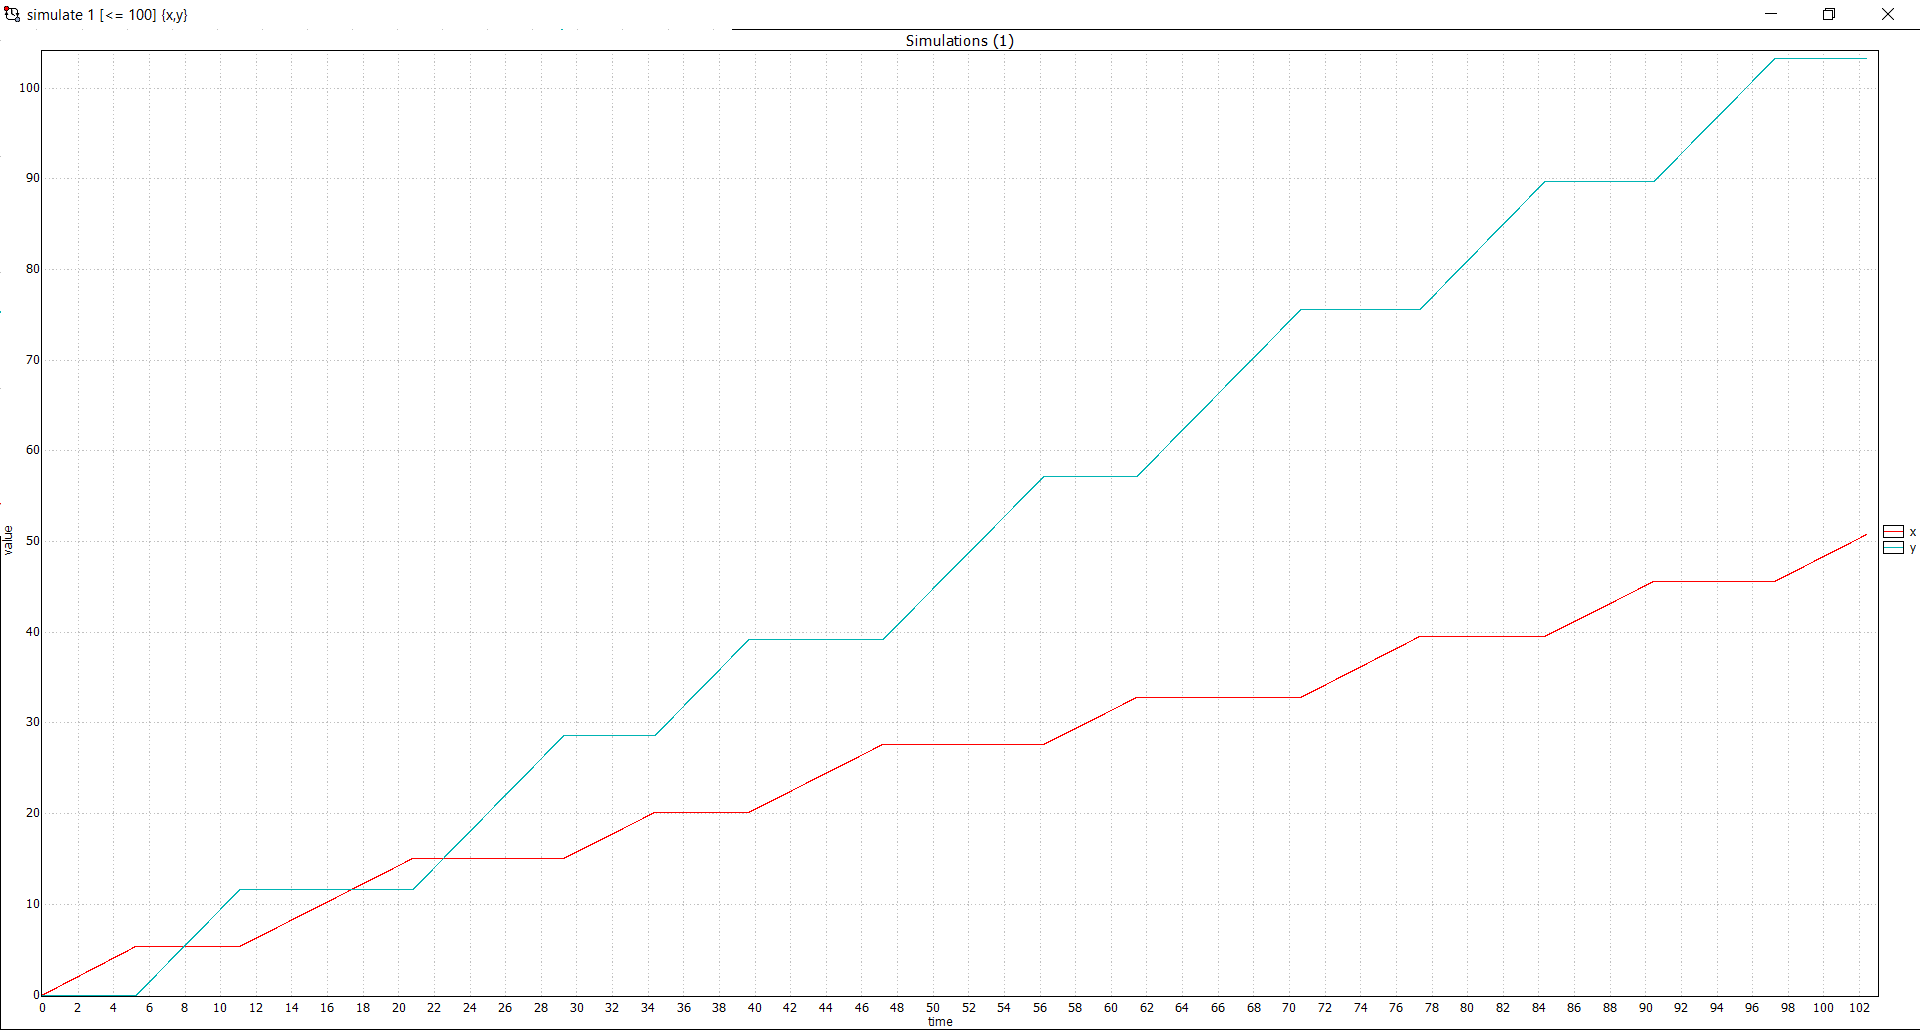
\includegraphics[width=\textwidth]{graphics/showcase01.png}
	\label{fig:sim01}
	\caption{One simulations of the value of two variables \uppVar{x, y} over 100 time units}
\end{figure}

\begin{figure}[!h]
	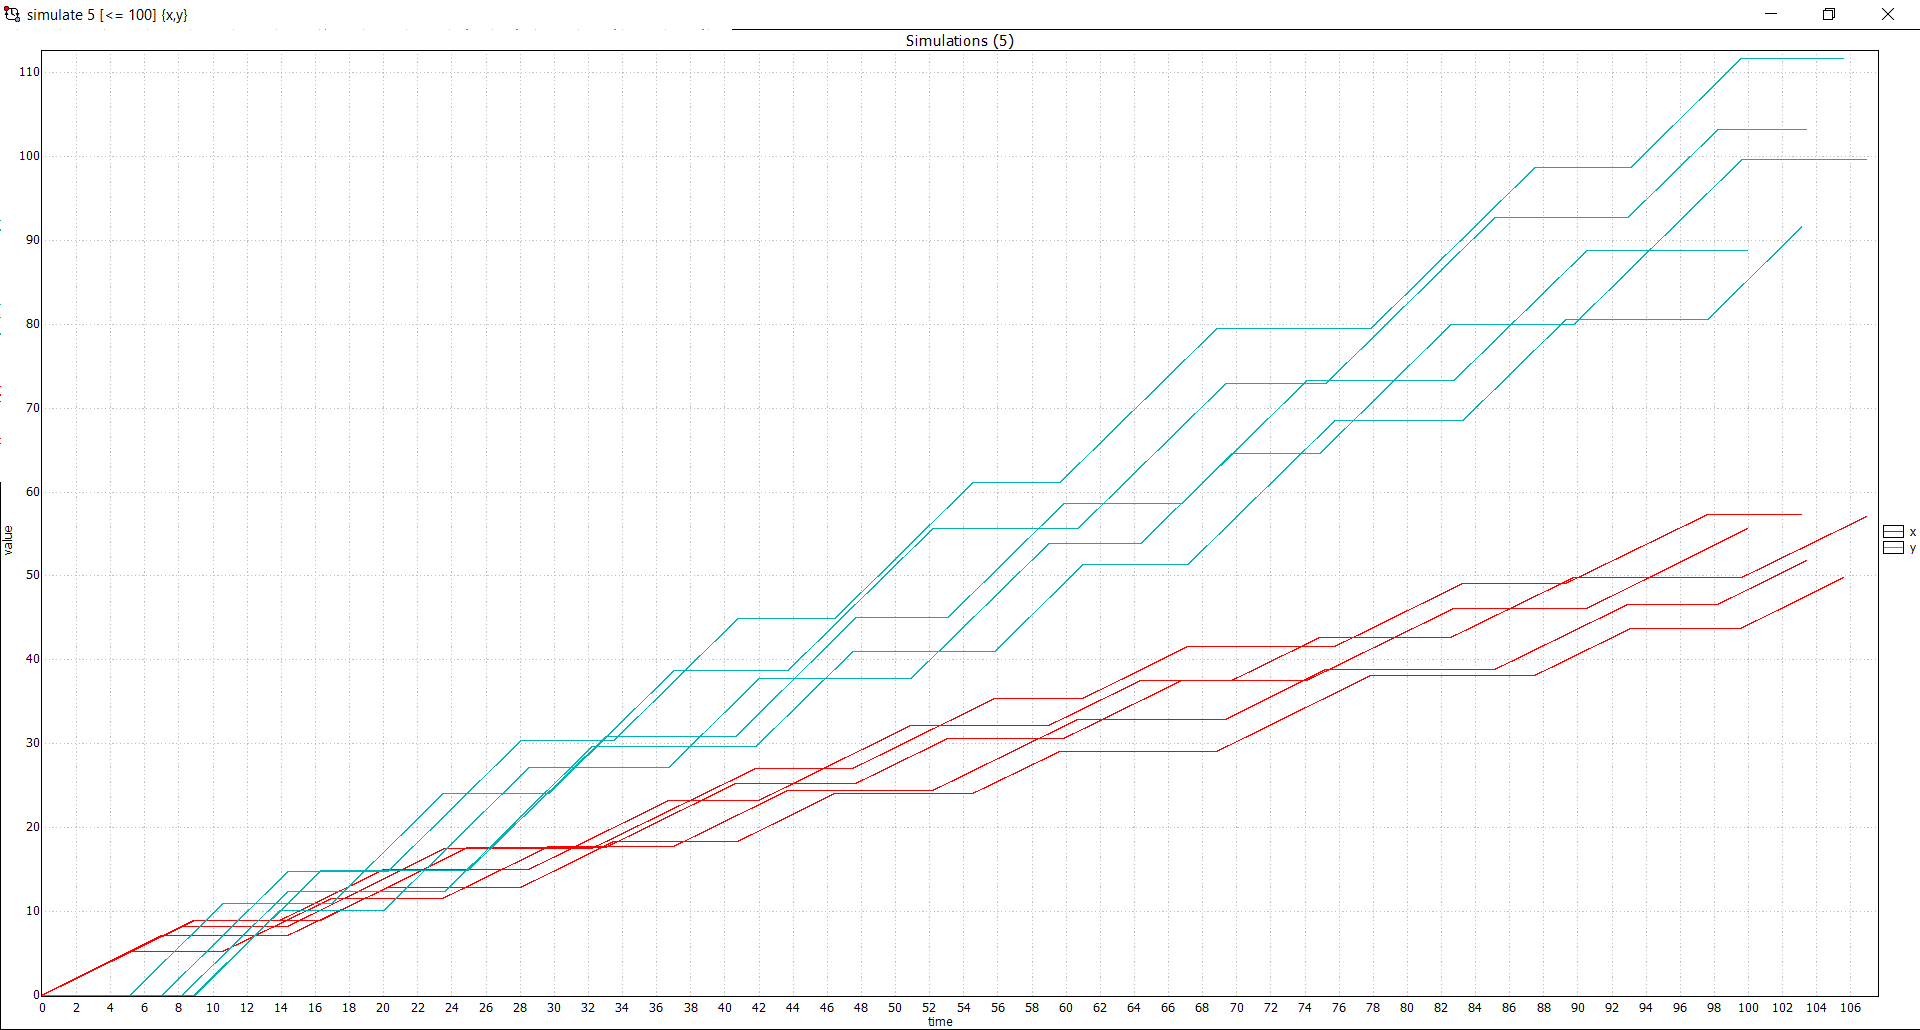
\includegraphics[width=\textwidth]{graphics/showcase02.png}
	\label{fig:sim02}
	\caption{Five simulations of the value of two variables \uppVar{x, y} over 100 time units}
\end{figure}

%TODO describe queries and afterwards the results.


%DEMO OF TIKZ
%\begin{figure}
%	\begin{tikzpicture}
%	\node [init] (start) {};
%	%\type [typeOfNode] (id) [relation from other nodes, distance, text] {text inside node}
%	\node [location] (end1) [right of=start, xshift=20mm, label={[align=left]below right:
%		\textcolor{name}{name}\\
%		\textcolor{invariant}{invariant}\\
%		\textcolor{RoE}{rate of expoential}
%	}] {$C$};
%	\node [location] (end2) [left of=start,xshift=-20mm] {$\cup$};
%	\path[->,black] (start) edge node [midway, below][align=left]{
%		\textcolor{select}{select}\\
%		\textcolor{guard}{guard}\\
%		\textcolor{sync}{sync}\\
%		\textcolor{update}{update}
%	} (end1);
%	\path[->,black] (start) edge node [midway, below][align=left]{
%		\textcolor{select}{select}\\
%		\textcolor{guard}{guard}\\
%		\textcolor{sync}{sync}\\
%		\textcolor{update}{update}
%	} (end2);
%	\end{tikzpicture}
%	\caption{Test example of UPPAAL models}
%	\label{fig:example1}
%\end{figure}

After having run a simulation query, it is possible to get a graph illustrating the result of running the simulations. In \cref{fig:simab} we see two variable which have been simulated five times for $15.000$ units of time, this will be useful for monitoring the battery energy levels over time.

\begin{figure}[!h]
	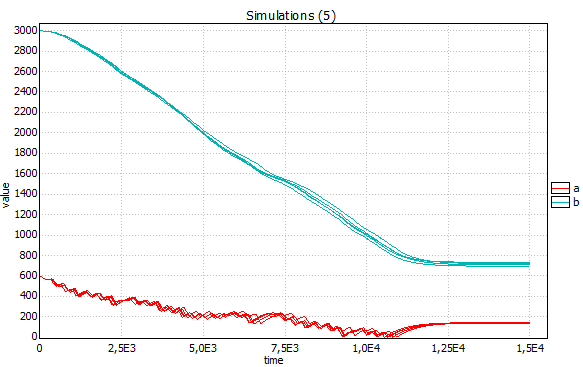
\includegraphics[width=\textwidth]{graphics/simab.png}
	\label{fig:simab}
	\caption{Five simulations of the value of two variables \uppVar{a, b} over time}
\end{figure}

Also it is possible to run probabilities queries, these answers the question; \textit{"What is the probability that some condition will be fulfilled?"}. An example of this can be seen in \cref{fig:pra300}, where we have run the probability that our variable \uppVar{a} will fall below $300$ within time $7200$ units of time. \Gls{smc} have then run this by randomly simulating the models behaviour until it with some certainty, within a specified margin of error, knows the chance of the property being true.\\
\Cref{fig:pra300} shows that prior to time $4120$ there are no chance of \uppVar{a} being under $300$, and at time $4520$ it will with certainty be under $300$. For this query it was specified that a $5\%$ uncertainty was acceptable, this resulted in the result seen in \cref{fig:pra300pct} which shows that \gls{smc} was $~90\% - 100\%$ certain \uppVar{a} would fall below $300$. The certainty parameter can be modified to become more precise, at the cost of run time as it will have to run more simulations in order to ensure the correct probability. Using the probability query also allow  for several other types graphs such as probability distribution and frequency histogram.

\begin{figure}[h]
	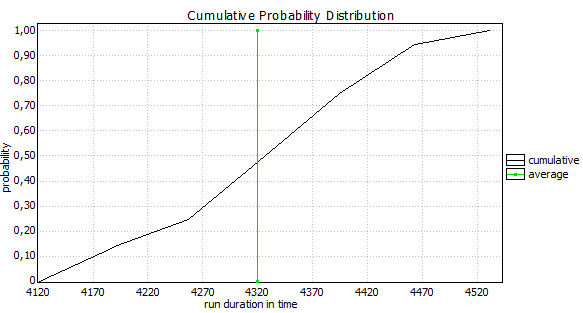
\includegraphics[width=\textwidth]{graphics/pra300.png}
	\label{fig:pra300}
	\caption{Probability over time that the value of (a) will fall under 300}
\end{figure}

\begin{figure}[h]
	\centering
	
\includegraphics[width=8cm]{graphics/pra300pct.png}
	\label{fig:pra300pct}
	\caption{Initial result of running a probability query}
\end{figure}


